\documentclass[11pt]{article}
\usepackage[margin=1in]{geometry}
\usepackage{amsmath,amssymb,amsthm}
\usepackage{graphicx}
\usepackage{microtype}
\usepackage[hidelinks]{hyperref}

\newtheorem{theorem}{Theorem}

\title{A Dense Incomplete Subspace with No Essential Schauder Basis\\
\large A candidate counterexample to both Problems 1 and 2 of arXiv:1806.07943}
\author{Automated mathematical discovery run \texttt{fa\_banach\_001}, lane 15}
\date{11 August 2026}

\begin{document}
\maketitle

\begin{center}
\fbox{\parbox{0.91\linewidth}{\textbf{Status.} Candidate full counterexample,
likely valid, requiring expert review. The bounded search described below
found no explicit later resolution.}}
\end{center}

\begin{abstract}
We answer both open problems of Coelho--Ribeiro--Salgado negatively. Let $B$
be a separable Banach space without a Schauder basis and let $X$ be the
algebraic span of a countable dense subset of $B$. Then $X$ is a separable,
proper, dense, incomplete normed subspace with completion $B$. The source
paper's own Banach--Grunblum criterion says that an essential Schauder basis
of $X$ would extend to a Schauder basis of $B$, which is impossible. Since an
essential unconditional basis is, by definition, an essential Schauder
basis, the same $X$ also answers the second problem negatively.
\end{abstract}

\section{The two source problems}

Coelho, Ribeiro, and Salgado ask whether every separable incomplete normed
space admits an essential Schauder basis, and whether every incomplete normed
space admits an essential unconditional basis \cite{source}.

\begin{figure}[ht]
  \centering
  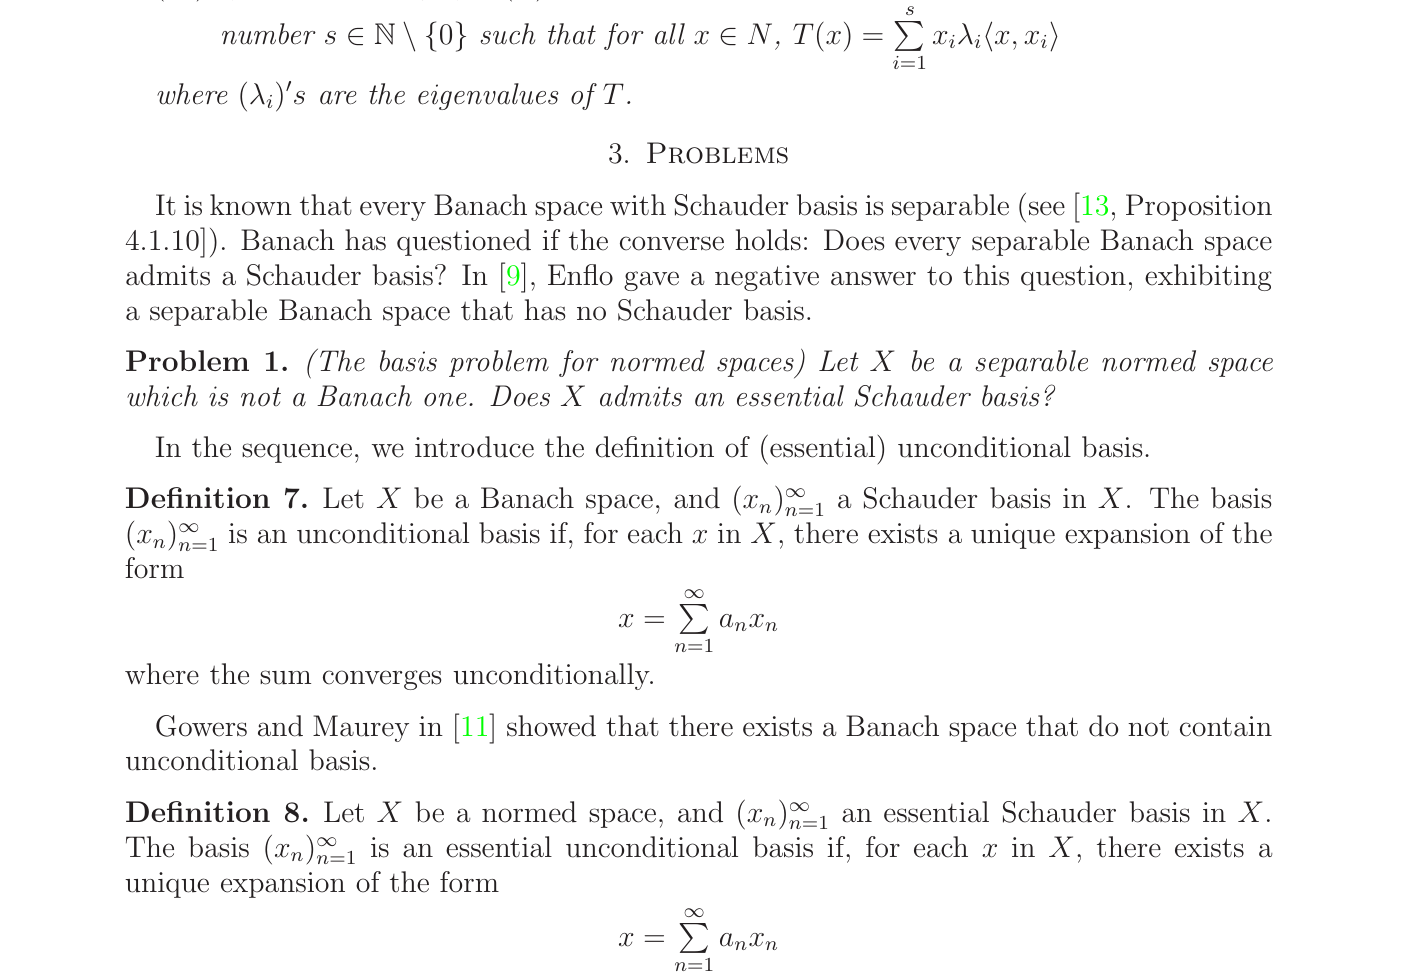
\includegraphics[width=0.96\linewidth]{figures/problem_1_crop.png}
  \caption{Problem 1 and its immediate context in the source, PDF p.~5.}
\end{figure}

\begin{figure}[ht]
  \centering
  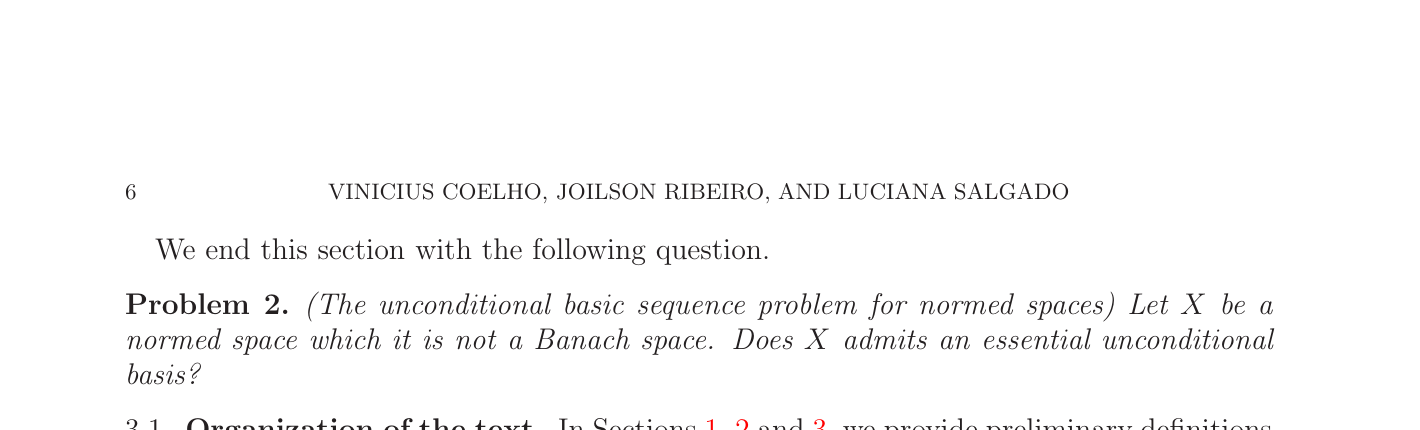
\includegraphics[width=0.96\linewidth]{figures/problem_2_crop.png}
  \caption{Problem 2 in the source, PDF p.~6.}
\end{figure}

\section{Definitions and the completion mechanism}

For a Schauder basis $(x_n)$ of a normed space $X$, the source calls it
\emph{essential} when the synthesis map from its convergent coefficient
space, equipped with the supremum norm of partial sums, onto $X$ is an
isomorphism. Its Theorem A states, in particular, that an essential basic
sequence in $X$ is an essential Schauder basis of the completion of its closed
linear span in the completion $\widehat X$ \cite{source}.

Consequently, if $(x_n)$ is an essential Schauder basis of all of $X$, then
the same sequence is a Schauder basis of $\widehat X$. The word
``essential'' adds nothing in the Banach space $\widehat X$, since every
Schauder basis of a Banach space is essential in the source's terminology.

\section{Proof intuition}

The obstruction to a basis can be placed entirely in the completion. Start
with a separable Banach space $B$ known to have no Schauder basis, but retain
only the algebraic span of a countable dense set. This produces an incomplete
space satisfying the source hypotheses without changing its completion.
Essentiality is exactly strong enough, by the source's Theorem A, to transport
any proposed basis back to that forbidden completion.

The unconditional question needs no separate convergence argument. Under the
source's Definition 8, ``essential unconditional'' is an additional property
of an already essential Schauder basis. The first obstruction therefore
settles both questions.

\section{Counterexample}

\begin{theorem}\label{thm:counterexample}
There exists a separable incomplete normed space $X$ which has neither an
essential Schauder basis nor an essential unconditional basis. Hence Problems
1 and 2 of \cite{source} both have negative answers.
\end{theorem}

\begin{proof}
Let $B$ be a separable infinite-dimensional Banach space without a Schauder
basis. Such a space exists by Enflo's construction of a separable Banach space
without the approximation property \cite{enflo}, since a Schauder basis gives
bounded finite-rank partial-sum projections converging pointwise to the
identity and hence the bounded approximation property.

Choose a countable dense set $D=\{d_1,d_2,\ldots\}$ in $B$ and put
\[
 X=\operatorname{span}D
\]
with the norm inherited from $B$. The space $X$ is separable and dense in
$B$. It is proper: otherwise $B$ would have countable Hamel dimension, hence
would be the union of the increasing finite-dimensional closed subspaces
$\operatorname{span}\{d_1,\ldots,d_m\}$. This contradicts the Baire category
theorem because $B$ is infinite-dimensional. Since a complete subspace of a
Banach space is closed, the proper dense subspace $X$ is incomplete. Its
completion is canonically isometric to $B$.

Suppose that $(x_n)$ were an essential Schauder basis of $X$. Then
$\overline{\operatorname{span}}^{\,X}\{x_n:n\geq1\}=X$. Applying item
(ii)$\Rightarrow$(i) of
Theorem A in \cite{source}, $(x_n)$ is an essential Schauder basis of the
completion of this closed span, namely $B$. Thus $B$ has a Schauder basis,
contrary to its choice. Therefore $X$ has no essential Schauder basis.

Finally, Definition 8 of \cite{source} defines an essential unconditional
basis to be an essential Schauder basis whose expansions converge
unconditionally. Since $X$ has no essential Schauder basis at all, it has no
essential unconditional basis. This same $X$ disproves both universal
statements.
\end{proof}

\section{Verification, limitations, and novelty}

The verification report checks separately: properness by Baire category,
incompleteness and identification of the completion, the exact application of
Theorem A, and the definitional implication for unconditional bases. No
finite computation is relevant.

The result is existential because it inherits the known Enflo space; it does
not provide a simpler concrete norm formula for $B$. It also does not classify
which incomplete normed spaces do possess essential bases.

A bounded search on 11 August 2026 covered the run's registry, solution,
attempt, and active-claim indexes; the exact arXiv id and title; both exact
problem phrases; the November 2024 arXiv/published version; and combinations
of dense subspaces, completions, Enflo spaces, and essential Schauder bases.
The current version still states both problems, and no explicit answer was
found. This is provisional novelty evidence only.

\section*{Human-review recommendation}

Check first that Theorem A of the source applies to a basis spanning all of
$X$, so its completed closed span is precisely $\widehat X=B$. Then verify
that Definition 8 makes the second conclusion immediate. The Baire-category
and completion steps are standard.

\enlargethispage{4\baselineskip}
\begin{thebibliography}{9}
\bibitem{source}
V. Coelho, J. Ribeiro, and L. Salgado,
\emph{A note on Basis Problem in normed spaces}, arXiv:1806.07943,
Problems 1--2 and Theorem A; published version, 2024.

\bibitem{enflo}
P. Enflo,
\emph{A counterexample to the approximation problem in Banach spaces},
Acta Math. \textbf{130} (1973), 309--317.
\end{thebibliography}

\end{document}
